% deepstudy-pdf — Guia Completo de Inglês para Comunicação (Partes 1–3)
\documentclass[12pt,a4paper,oneside]{book}
\usepackage[utf8]{inputenc}
\usepackage[T1]{fontenc}
\usepackage{amsmath,amssymb}
\usepackage{listings}
\usepackage{xcolor}
\usepackage{hyperref}
\usepackage{tikz}
\usetikzlibrary{arrows.meta}
\usetikzlibrary{shapes.geometric}
\usetikzlibrary{positioning}
\usepackage{minted}
\usepackage{tcolorbox}
\usepackage{geometry}
\usepackage{fancyhdr}
\usepackage{imakeidx}
\usepackage{booktabs}
\usepackage{tabularx}
\usepackage{array}
\usepackage{float}

\makeindex[intoc]

\geometry{margin=2.5cm}
\setlength{\parskip}{0.8em}
\setlength{\parindent}{0pt}
\setlength{\headheight}{14.5pt}

\pagestyle{fancy}
\fancyhf{}
\fancyhead[LE,RO]{\thepage}
\fancyhead[RE]{\nouppercase{\leftmark}}
\fancyhead[LO]{\nouppercase{\rightmark}}

\hypersetup{
    colorlinks=true,
    linkcolor=blue!60!black,
    urlcolor=blue!60!black,
    citecolor=blue!60!black,
}

% ---- macros e caixas ----
\newcommand{\en}[1]{\textit{#1}}                 % frase em inglês
\newcommand{\aux}[1]{\textbf{\textcolor{blue!60!black}{#1}}} % auxiliar destacado
\newcommand{\blank}{\underline{\hspace{1.4cm}}}
\newcommand{\ok}{\textcolor{green!45!black}{$\checkmark$}}
\newcommand{\no}{\textcolor{red!70!black}{$\times$}}
\newcommand{\ra}{$\rightarrow$}
\newcommand{\fr}[2]{\en{#1} & #2 \\}
\newenvironment{frases}{\tabularx{\textwidth}{@{}>{\raggedright\arraybackslash}p{0.52\textwidth}X@{}}}{\endtabularx}
\newcommand{\estrutura}[1]{\begin{center}\fbox{\parbox{0.85\textwidth}{\centering\sffamily\bfseries #1}}\end{center}}

\newtcolorbox{nota}[1][Nota]{colback=blue!3,colframe=blue!50!black,title={#1},fonttitle=\bfseries,boxrule=0.6pt,arc=2pt}
\newtcolorbox{cuidado}[1][Atenção]{colback=orange!5,colframe=orange!70!black,title={#1},fonttitle=\bfseries,boxrule=0.6pt,arc=2pt}
\newtcolorbox{pratica}[1][Na prática]{colback=green!4,colframe=green!45!black,title={#1},fonttitle=\bfseries,boxrule=0.6pt,arc=2pt}

\tikzset{
  caixa/.style={draw, rounded corners=2pt, fill=gray!8, align=center, text width=#1, inner sep=4pt, minimum height=0.65cm, font=\small},
  caixa/.default=2.4cm,
  destaque/.style={draw=blue!60!black, rounded corners=2pt, fill=blue!8, align=center, text width=#1, inner sep=4pt, minimum height=0.65cm, font=\small\bfseries},
  destaque/.default=2.4cm,
  seta/.style={-Stealth, thick},
}

\title{Guia Completo de Inglês para Comunicação\\[0.4em]\Large Do básico ao dia a dia --- explicado em português}
\author{DeepStudy PDF Generator}
\date{\today}

\begin{document}

\maketitle
\tableofcontents

% =====================================================================
\chapter*{Como usar este guia}
\addcontentsline{toc}{chapter}{Como usar este guia}
\markboth{Como usar este guia}{Como usar este guia}

Este guia cobre o núcleo de qualquer conversa: \textbf{perguntar}, \textbf{responder} e \textbf{pedir} (Capítulos 1--3). Quase toda interação do dia a dia --- no restaurante, no trabalho, na rua --- é uma combinação dessas três coisas. Em seguida vêm \textbf{falar sobre coisas} (descrever, tempos verbais, opinião), \textbf{situações reais} (restaurante, aeroporto, hotel, compras, médico, trabalho), os \textbf{erros típicos de brasileiros}, um \textbf{vocabulário essencial} e \textbf{exercícios com gabarito}.

\begin{itemize}
  \item Frases em inglês aparecem em \en{itálico}; a tradução vem ao lado.
  \item Auxiliares (a peça que faz a pergunta funcionar) aparecem em \aux{azul e negrito}.
  \item Caixas \textbf{Atenção} marcam os erros mais comuns de brasileiros.
  \item Caixas \textbf{Na prática} trazem frases prontas para decorar.
  \item O Capítulo~\ref{cap:revisao} resume tudo nas 10 regras de ouro; o glossário e o índice remissivo estão no final.
\end{itemize}

\begin{nota}[A ideia central do guia]
Em português, a entonação faz quase todo o trabalho. Em inglês, é a \textbf{ordem das palavras} que faz. Se você entender \emph{onde o auxiliar entra}, 80\% das perguntas, respostas curtas, \emph{question tags} e pedidos passam a seguir a mesma lógica.
\end{nota}

% =====================================================================
\chapter{Como Fazer Perguntas}
\label{cap:perguntas}

\section{A lógica das perguntas em inglês}

Em português, muitas vezes a gente só muda a entonação: ``Você fala inglês.'' vira ``Você fala inglês?'' apenas pelo tom de voz. Em inglês, isso quase nunca funciona. O inglês precisa de \textbf{estrutura} para fazer pergunta: uma palavra extra (o auxiliar) e uma mudança na ordem das palavras.

Existem dois grandes tipos de pergunta:

\begin{center}
\begin{tabularx}{\textwidth}{@{}lXl@{}}
\toprule
\textbf{Tipo} & \textbf{Resposta esperada} & \textbf{Exemplo} \\
\midrule
\en{Yes/No questions}\index{Yes/No question} & Sim ou não & \en{Do you speak English?} \\
\en{WH- questions}\index{WH- question} & Uma informação & \en{Where do you live?} \\
\bottomrule
\end{tabularx}
\end{center}

% ---------------------------------------------------------------------
\section{Yes/No questions (perguntas de sim ou não)}

\subsection{A estrutura básica}

\estrutura{Auxiliar + Sujeito + Verbo principal + Complemento ?}

O \textbf{auxiliar}\index{auxiliar} é a peça-chave. Ele vem \textbf{antes do sujeito}. É isso que transforma uma frase afirmativa em pergunta. Há dois casos:

\begin{enumerate}
  \item A frase \textbf{já tem} um auxiliar (\en{is}, \en{can}, \en{will}\ldots): ele simplesmente \textbf{troca de lugar} com o sujeito (\emph{inversão}\index{inversão}).
  \item A frase \textbf{não tem} auxiliar (verbo comum no presente ou passado): você \textbf{insere} \aux{do}, \aux{does} ou \aux{did}.
\end{enumerate}

\begin{figure}[H]
\centering
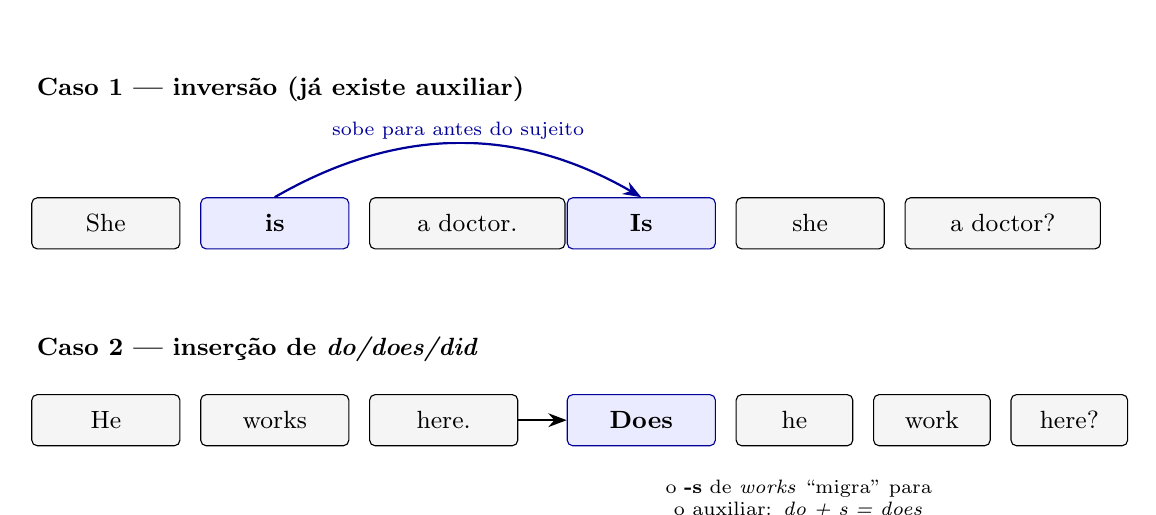
\begin{tikzpicture}[node distance=0.25cm]
  % Caso 1: inversão
  \node[font=\small\bfseries, anchor=west] at (-0.2,3.7) {Caso 1 --- inversão (já existe auxiliar)};
  \node[caixa=1.6cm] (s1) at (0.8,2) {She};
  \node[destaque=1.6cm, right=of s1] (a1) {is};
  \node[caixa=2.2cm, right=of a1] (c1) {a doctor.};
  \node[destaque=1.6cm] (a1b) at (7.6,2) {Is};
  \node[caixa=1.6cm, right=of a1b] (s1b) {she};
  \node[caixa=2.2cm, right=of s1b] (c1b) {a doctor?};
  \draw[seta, blue!60!black] (a1.north) to[bend left=30] node[above, font=\scriptsize, fill=white, inner sep=1pt]{sobe para antes do sujeito} (a1b.north);

  % Caso 2: inserção
  \node[font=\small\bfseries, anchor=west] at (-0.2,0.4) {Caso 2 --- inserção de \emph{do/does/did}};
  \node[caixa=1.6cm] (s2) at (0.8,-0.5) {He};
  \node[caixa=1.6cm, right=of s2] (v2) {works};
  \node[caixa=1.6cm, right=of v2] (c2) {here.};
  \node[destaque=1.6cm] (a2b) at (7.6,-0.5) {Does};
  \node[caixa=1.2cm, right=of a2b] (s2b) {he};
  \node[caixa=1.2cm, right=of s2b] (v2b) {work};
  \node[caixa=1.2cm, right=of v2b] (c2b) {here?};
  \draw[seta] (c2.east) -- (a2b.west);
  \node[font=\scriptsize, text width=4.2cm, align=center] at (9.6,-1.5) {o \textbf{-s} de \en{works} ``migra'' para o auxiliar: \en{do + s = does}};
\end{tikzpicture}
\caption{As duas formas de montar uma \emph{Yes/No question}.}
\end{figure}

\subsection{Os auxiliares mais usados}

\begin{center}
\begin{tabularx}{\textwidth}{@{}lXl@{}}
\toprule
\textbf{Auxiliar} & \textbf{Quando usar} & \textbf{Exemplo} \\
\midrule
\aux{Do}\index{do/does/did} & Presente, com I/You/We/They & \en{Do you like pizza?} \\
\aux{Does} & Presente, com He/She/It & \en{Does she work here?} \\
\aux{Did} & Passado (todas as pessoas) & \en{Did you call him?} \\
\aux{Am / Is / Are}\index{verbo to be} & Verbo \en{to be} no presente & \en{Are you tired?} \\
\aux{Was / Were} & Verbo \en{to be} no passado & \en{Was he at home?} \\
\aux{Have / Has}\index{present perfect} & \en{Present perfect} & \en{Have you seen this?} \\
\aux{Will} & Futuro & \en{Will you come?} \\
\aux{Can}\index{modal verb} & Habilidade / permissão & \en{Can you help me?} \\
\aux{Could} & Pedido educado / possibilidade & \en{Could you repeat?} \\
\aux{Should} & Conselho & \en{Should I go?} \\
\aux{Would} & Pedido educado / hipótese & \en{Would you like coffee?} \\
\bottomrule
\end{tabularx}
\end{center}

\subsection{Afirmação \ra\ pergunta, lado a lado}

\begin{center}
\begin{tabularx}{\textwidth}{@{}lXX@{}}
\toprule
\textbf{Grupo} & \textbf{Afirmação} & \textbf{Pergunta} \\
\midrule
\en{To be} (ser/estar) & \en{You are happy.} & \en{\aux{Are} you happy?} \\
 & \en{She is a doctor.} & \en{\aux{Is} she a doctor?} \\
 & \en{They were late.} & \en{\aux{Were} they late?} \\
\midrule
Presente (verbos comuns) & \en{You speak English.} & \en{\aux{Do} you speak English?} \\
 & \en{He works here.} & \en{\aux{Does} he work here?} \\
\midrule
Passado & \en{You called me.} & \en{\aux{Did} you call me?} \\
\midrule
Futuro & \en{You will travel.} & \en{\aux{Will} you travel?} \\
\midrule
\en{Can / Could} & \en{You can swim.} & \en{\aux{Can} you swim?} \\
\bottomrule
\end{tabularx}
\end{center}

\begin{cuidado}[Atenção: o auxiliar ``rouba'' a conjugação]
\begin{itemize}
  \item Com \aux{does}, o verbo perde o ``s'': \en{Does he \textbf{work}?} --- e não \en{works}.
  \item Com \aux{did}, o verbo volta à forma base\index{forma base}: \en{Did you \textbf{call}?} --- e não \en{called}.
\end{itemize}
Regra mental: \textbf{só uma palavra carrega o tempo verbal}. Se o auxiliar já mostra presente-3ª-pessoa ou passado, o verbo principal fica ``cru''.
\end{cuidado}

\subsection{Erros comuns de brasileiros}

\begin{center}
\begin{tabularx}{\textwidth}{@{}llX@{}}
\toprule
\textbf{\no\ Errado} & \textbf{\ok\ Certo} & \textbf{Por quê} \\
\midrule
\en{You speak English?} & \en{Do you speak English?} & Falta o auxiliar \\
\en{Does he works here?} & \en{Does he work here?} & ``s'' duplicado (auxiliar e verbo) \\
\en{Did you called?} & \en{Did you call?} & Passado duplicado com \en{did} \\
\en{Is you happy?} & \en{Are you happy?} & Concordância errada (\en{you} $\to$ \en{are}) \\
\bottomrule
\end{tabularx}
\end{center}

\begin{nota}[E ``You speak English?'' nunca é usado?]
Em conversa informal, nativos às vezes fazem pergunta só com entonação (\en{You're leaving already?}) --- mas para \textbf{expressar surpresa} ou confirmar algo que acabaram de ouvir, não como pergunta neutra. Para quem está aprendendo, a regra segura é: \textbf{sempre use o auxiliar}.
\end{nota}

% ---------------------------------------------------------------------
\section{WH- questions (perguntas com informação)}

\subsection{As palavras WH-}

\begin{center}
\begin{tabularx}{\textwidth}{@{}llX@{}}
\toprule
\textbf{Palavra} & \textbf{Significado} & \textbf{Uso} \\
\midrule
\en{What}\index{what} & O quê / Qual & Coisas, ações \\
\en{Where}\index{where} & Onde & Lugares \\
\en{When}\index{when} & Quando & Tempo \\
\en{Who}\index{who} & Quem & Pessoas (sujeito ou objeto, informal) \\
\en{Whom}\index{whom} & Quem & Pessoas (objeto --- formal) \\
\en{Whose}\index{whose} & De quem & Posse \\
\en{Why}\index{why} & Por que & Motivo \\
\en{Which}\index{which} & Qual & Escolha entre opções conhecidas \\
\en{How}\index{how} & Como & Modo, maneira \\
\bottomrule
\end{tabularx}
\end{center}

\subsection{A estrutura básica}

\estrutura{WH-word + Auxiliar + Sujeito + Verbo + Complemento ?}

A boa notícia: uma \emph{WH- question} é só uma \emph{Yes/No question} com a palavra interrogativa colada na frente.

\begin{figure}[H]
\centering
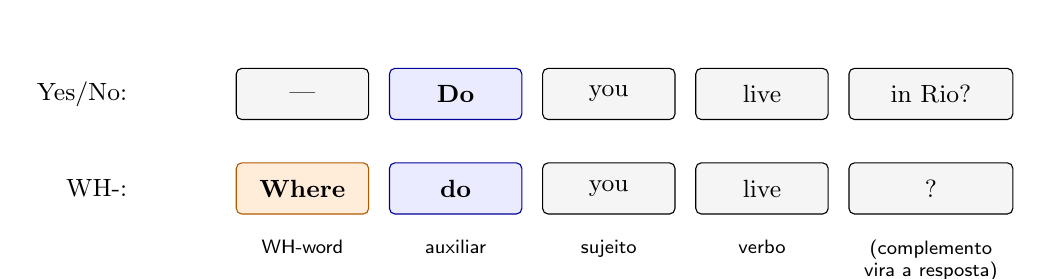
\begin{tikzpicture}[node distance=0.25cm]
  \node[font=\small, anchor=east] at (-0.1,1.2) {Yes/No:};
  \node[caixa=1.4cm] (y1) at (2.0,1.2) {---};
  \node[destaque=1.4cm, right=of y1] (y2) {Do};
  \node[caixa=1.4cm, right=of y2] (y3) {you};
  \node[caixa=1.4cm, right=of y3] (y4) {live};
  \node[caixa=1.8cm, right=of y4] (y5) {in Rio?};

  \node[font=\small, anchor=east] at (-0.1,0) {WH-:};
  \node[destaque=1.4cm, fill=orange!15, draw=orange!70!black] (w1) at (2.0,0) {Where};
  \node[destaque=1.4cm, right=of w1] (w2) {do};
  \node[caixa=1.4cm, right=of w2] (w3) {you};
  \node[caixa=1.4cm, right=of w3] (w4) {live};
  \node[caixa=1.8cm, right=of w4] (w5) {?};

  \node[font=\scriptsize\sffamily, below=0.2cm of w1] {WH-word};
  \node[font=\scriptsize\sffamily, below=0.2cm of w2] {auxiliar};
  \node[font=\scriptsize\sffamily, below=0.2cm of w3] {sujeito};
  \node[font=\scriptsize\sffamily, below=0.2cm of w4] {verbo};
  \node[font=\scriptsize\sffamily, below=0.2cm of w5, text width=2.2cm, align=center] {(complemento vira a resposta)};
\end{tikzpicture}
\caption{A WH-word ocupa o lugar da informação que você quer descobrir.}
\end{figure}

\subsection{Exemplos por palavra}

\textbf{WHAT} (O quê / Qual)

\begin{frases}
\fr{What \aux{do} you do?}{O que você faz? (profissão)}
\fr{What \aux{is} your name?}{Qual é o seu nome?}
\fr{What \aux{did} you eat?}{O que você comeu?}
\fr{What \aux{are} you doing?}{O que você está fazendo?}
\fr{What time \aux{is} it?}{Que horas são?}
\end{frases}

\textbf{WHERE} (Onde)

\begin{frases}
\fr{Where \aux{do} you live?}{Onde você mora?}
\fr{Where \aux{is} the bathroom?}{Onde é o banheiro?}
\fr{Where \aux{did} you go?}{Onde você foi?}
\fr{Where \aux{are} you from?}{De onde você é?}
\end{frases}

\textbf{WHEN} (Quando)

\begin{frases}
\fr{When \aux{do} you wake up?}{Quando você acorda?}
\fr{When \aux{is} your birthday?}{Quando é seu aniversário?}
\fr{When \aux{did} you arrive?}{Quando você chegou?}
\end{frases}

\textbf{WHO} (Quem)

\begin{frases}
\fr{Who \aux{is} that?}{Quem é aquele?}
\fr{Who called you?}{Quem te ligou?}
\end{frases}

\begin{cuidado}[Atenção: \emph{who} como sujeito não leva auxiliar]
Quando \en{who} (ou \en{what}) \textbf{é o sujeito} da frase --- ou seja, é quem faz a ação ---, não há inversão nem auxiliar:
\begin{itemize}
  \item \ok\ \en{Who called you?} (alguém te ligou; quem?) --- \no\ \en{Who did called you?}
  \item Compare: \en{Who \aux{did} you call?} = Para quem \emph{você} ligou? Aqui \en{you} é o sujeito, e \en{who} é o objeto\index{pergunta de sujeito}.
\end{itemize}
\end{cuidado}

\textbf{WHY} (Por que)

\begin{frases}
\fr{Why \aux{are} you sad?}{Por que você está triste?}
\fr{Why \aux{did} you do that?}{Por que você fez isso?}
\end{frases}

\textbf{WHICH} (Qual --- entre opções)

\begin{frases}
\fr{Which one \aux{do} you want?}{Qual você quer?}
\fr{Which color \aux{do} you prefer?}{Qual cor você prefere?}
\end{frases}

\begin{nota}[\emph{What} ou \emph{Which}?]
Use \en{which} quando há um conjunto limitado e conhecido de opções (``este ou aquele?''). Use \en{what} quando a pergunta é aberta: \en{What color is your car?} (qualquer cor) vs.\ \en{Which color do you prefer, red or blue?}
\end{nota}

\textbf{HOW} (Como)

\begin{frases}
\fr{How \aux{are} you?}{Como você está?}
\fr{How \aux{do} you spell it?}{Como se escreve isso?}
\fr{How old \aux{are} you?}{Quantos anos você tem?}
\end{frases}

\subsection{Combinações com HOW (muito usadas!)}

\begin{center}
\begin{tabularx}{\textwidth}{@{}lXl@{}}
\toprule
\textbf{Expressão} & \textbf{Significado} & \textbf{Exemplo} \\
\midrule
\en{How much}\index{how much / how many} & Quanto (incontável / preço) & \en{How much is it?} \\
\en{How many} & Quantos (contável) & \en{How many people?} \\
\en{How long} & Quanto tempo & \en{How long does it take?} \\
\en{How far} & Quão longe & \en{How far is the hotel?} \\
\en{How often} & Com que frequência & \en{How often do you study?} \\
\en{How old} & Quantos anos & \en{How old is he?} \\
\bottomrule
\end{tabularx}
\end{center}

% ---------------------------------------------------------------------
\section{Question tags (perguntas de confirmação)}

São aquelas ``né?'', ``não é?'' no final da frase. Servem para confirmar algo que você já acha que é verdade\index{question tag}.

\textbf{Regra:} se a frase é \textbf{afirmativa}, a tag é \textbf{negativa}. Se a frase é \textbf{negativa}, a tag é \textbf{afirmativa}. A tag sempre repete o \textbf{mesmo auxiliar} da frase (ou \en{do/does/did}, se a frase não tiver um).

\begin{figure}[H]
\centering
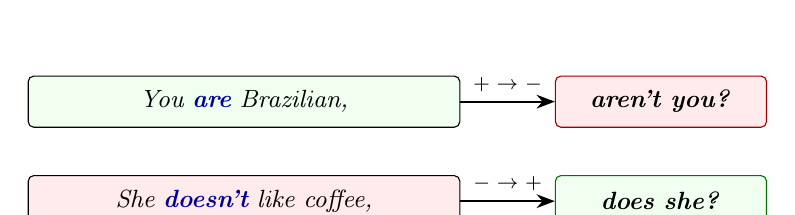
\begin{tikzpicture}[node distance=0.3cm]
  \node[caixa=5.2cm, fill=green!6] (p1) {\en{You \aux{are} Brazilian,}};
  \node[destaque=2.4cm, fill=red!8, draw=red!60!black, right=1.2cm of p1] (t1) {\en{aren't you?}};
  \draw[seta] (p1) -- node[above, font=\scriptsize]{$+ \to -$} (t1);

  \node[caixa=5.2cm, fill=red!8, below=0.6cm of p1] (p2) {\en{She \aux{doesn't} like coffee,}};
  \node[destaque=2.4cm, fill=green!6, draw=green!45!black, right=1.2cm of p2] (t2) {\en{does she?}};
  \draw[seta] (p2) -- node[above, font=\scriptsize]{$- \to +$} (t2);
\end{tikzpicture}
\caption{A polaridade da tag é sempre oposta à da frase.}
\end{figure}

\begin{frases}
\fr{You are Brazilian, aren't you?}{Você é brasileiro, não é?}
\fr{She doesn't like coffee, does she?}{Ela não gosta de café, gosta?}
\fr{You went there, didn't you?}{Você foi lá, não foi?}
\fr{He can swim, can't he?}{Ele sabe nadar, não sabe?}
\end{frases}

Repare em \en{You \textbf{went} there, \textbf{didn't} you?}: a frase não tem auxiliar visível, então a tag usa \aux{did} (porque \en{went} é passado).

% ---------------------------------------------------------------------
\section{Indirect questions (perguntas indiretas --- mais educadas)}

Quando você quer ser mais educado, começa com uma frase introdutória e a pergunta original ``vira afirmação''\index{indirect question}.

\begin{center}
\begin{tabular}{@{}ll@{}}
\toprule
\textbf{Direta} & \en{Where \aux{is} the station?} \\
\textbf{Indireta} & \en{Could you tell me where the station \aux{is}?} \\
\bottomrule
\end{tabular}
\end{center}

\begin{cuidado}[Atenção: na pergunta indireta, o sujeito volta para antes do verbo]
\begin{itemize}
  \item \no\ \en{Do you know where is he?}
  \item \ok\ \en{Do you know where he is?}
\end{itemize}
A ``pergunta de verdade'' já está no começo (\en{Do you know\ldots?}). O resto volta à ordem normal de afirmação --- e \en{do/does/did} desaparecem: \en{Where \textbf{does} she live?} \ra\ \en{Do you know where she \textbf{lives}?}
\end{cuidado}

\textbf{Frases introdutórias comuns:} \en{Could you tell me\ldots}, \en{Do you know\ldots}, \en{I was wondering\ldots}, \en{Can I ask you\ldots}

\begin{frases}
\fr{Could you tell me what time it is?}{Você poderia me dizer que horas são?}
\fr{Do you know how to get there?}{Você sabe como chegar lá?}
\fr{I was wondering if you could help me.}{Eu queria saber se você poderia me ajudar.}
\end{frases}

Para transformar uma \emph{Yes/No question} em indireta, use \en{if} (ou \en{whether}): \en{Is the museum open?} \ra\ \en{Do you know \textbf{if} the museum is open?}

% ---------------------------------------------------------------------
\section{Perguntas do dia a dia (para memorizar)}

\begin{pratica}[Cumprimentos e \emph{small talk}]
\begin{frases}
\fr{How are you doing?}{Como vai?}
\fr{What's up?}{E aí? (informal)}
\fr{How's it going?}{Como estão as coisas?}
\fr{What have you been up to?}{O que você tem feito?}
\end{frases}
\end{pratica}

\begin{pratica}[Sobre a pessoa]
\begin{frases}
\fr{Where are you from?}{De onde você é?}
\fr{What do you do for a living?}{O que você faz da vida?}
\fr{How old are you?}{Quantos anos você tem?}
\fr{Are you married?}{Você é casado(a)?}
\end{frases}
\end{pratica}

\begin{pratica}[No dia a dia]
\begin{frases}
\fr{Can you help me?}{Você pode me ajudar?}
\fr{What does this mean?}{O que isso significa?}
\fr{How do you say \blank\ in English?}{Como se diz \blank\ em inglês?}
\fr{Can you repeat that, please?}{Você pode repetir, por favor?}
\end{frases}
\end{pratica}

\begin{nota}[Cuidado cultural]
\en{How old are you?} e \en{Are you married?} são gramaticalmente simples, mas em muitos países de língua inglesa soam invasivas vindas de um desconhecido. Guarde para quando já houver intimidade.
\end{nota}

% =====================================================================
\chapter{Como Responder Perguntas}
\label{cap:respostas}

\section{Short answers (respostas curtas)}

Em inglês é muito comum responder com \textbf{respostas curtas}\index{short answer}: não precisa repetir a frase toda, e também não se responde só ``sim'' ou ``não''.

\estrutura{Yes / No + sujeito + auxiliar (o mesmo da pergunta)}

\begin{figure}[H]
\centering
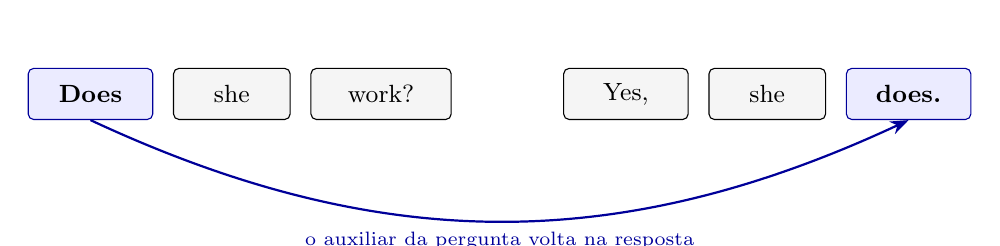
\begin{tikzpicture}[node distance=0.25cm]
  \node[destaque=1.3cm] (q1) at (0,0) {Does};
  \node[caixa=1.2cm, right=of q1] (q2) {she};
  \node[caixa=1.5cm, right=of q2] (q3) {work?};
  \node[caixa=1.3cm] (r1) at (6.8,0) {Yes,};
  \node[caixa=1.2cm, right=of r1] (r2) {she};
  \node[destaque=1.3cm, right=of r2] (r3) {does.};
  \draw[seta, blue!60!black] (q1.south) to[bend right=25] node[below, font=\scriptsize]{o auxiliar da pergunta volta na resposta} (r3.south);
\end{tikzpicture}
\caption{A resposta curta ``devolve'' o auxiliar da pergunta.}
\end{figure}

\begin{center}
\begin{tabularx}{\textwidth}{@{}XXX@{}}
\toprule
\textbf{Pergunta} & \textbf{Afirmativa} & \textbf{Negativa} \\
\midrule
\en{Do you like pizza?} & \en{Yes, I do.} & \en{No, I don't.} \\
\en{Does she work?} & \en{Yes, she does.} & \en{No, she doesn't.} \\
\en{Did you call?} & \en{Yes, I did.} & \en{No, I didn't.} \\
\en{Are you tired?} & \en{Yes, I am.} & \en{No, I'm not.} \\
\en{Is he here?} & \en{Yes, he is.} & \en{No, he isn't.} \\
\en{Were they late?} & \en{Yes, they were.} & \en{No, they weren't.} \\
\en{Can you swim?} & \en{Yes, I can.} & \en{No, I can't.} \\
\en{Will you come?} & \en{Yes, I will.} & \en{No, I won't.} \\
\en{Have you seen it?} & \en{Yes, I have.} & \en{No, I haven't.} \\
\bottomrule
\end{tabularx}
\end{center}

\begin{cuidado}[Atenção: ``Yes'' ou ``No'' sozinho soa seco]
Responder só \en{Yes} ou \en{No} costuma parecer seco ou até grosseiro. Sempre que possível, use a resposta curta completa.

Detalhe técnico: na afirmativa \textbf{não se contrai} o final --- \no\ \en{Yes, I'm.} / \ok\ \en{Yes, I am.}; \no\ \en{Yes, he's.} / \ok\ \en{Yes, he is.} Na negativa, a contração é o normal (\en{No, I'm not}, \en{No, he isn't}).
\end{cuidado}

\section{Respostas longas (quando quer dar mais informação)}

Depois do \en{Yes/No} + auxiliar, você pode emendar uma frase com detalhes. Isso mantém a conversa viva.

\begin{frases}
\fr{Do you like pizza?}{\en{Yes, I do. I love it, especially with pepperoni.}}
\fr{Did you go to the party?}{\en{No, I didn't. I was too tired.}}
\fr{Can you help me?}{\en{Sure, I can. What do you need?}}
\end{frases}

\section{Como responder perguntas WH-}

Aqui não existe ``sim ou não''. Você responde \textbf{direto com a informação} --- em geral reaproveitando o verbo da pergunta.

\begin{frases}
\fr{Where do you live?}{\en{I live in São Paulo.}}
\fr{What do you do?}{\en{I'm a teacher.} / \en{I work as a teacher.}}
\fr{Why are you late?}{\en{Because the traffic was terrible.}}
\fr{How are you?}{\en{I'm fine, thanks. And you?}}
\end{frases}

Repare: a pergunta usa \en{\aux{do} you live}, mas a resposta é \en{I \textbf{live}} --- o \en{do} só existe na pergunta.

\begin{pratica}[Conectores úteis para responder]
\begin{frases}
\fr{Because\ldots}{Porque\ldots}
\fr{Well\ldots}{Bem\ldots}
\fr{Actually\ldots}{Na verdade\ldots}
\fr{I think\ldots}{Eu acho\ldots}
\fr{In my opinion\ldots}{Na minha opinião\ldots}
\fr{Let me think\ldots}{Deixa eu pensar\ldots}
\end{frases}
\end{pratica}

\begin{nota}[\emph{Actually} é falso cognato]
\en{Actually}\index{actually} \textbf{não} significa ``atualmente'' --- significa ``na verdade'', ``na real''. ``Atualmente'' é \en{currently} ou \en{nowadays}.
\end{nota}

\section{Como responder quando NÃO sabe}

Muito importante! Nem sempre você vai saber responder --- e saber \emph{dizer que não entendeu} é o que salva a conversa.

\begin{pratica}[Frases de sobrevivência]
\begin{frases}
\fr{I don't know.}{Eu não sei.}
\fr{I'm not sure.}{Não tenho certeza.}
\fr{I have no idea.}{Não faço ideia.}
\fr{Sorry, I don't understand.}{Desculpa, não entendi.}
\fr{Could you repeat that, please?}{Pode repetir, por favor?}
\fr{Could you speak more slowly?}{Pode falar mais devagar?}
\fr{What does \blank\ mean?}{O que significa \blank?}
\fr{How do you say \blank\ in English?}{Como se diz \blank\ em inglês?}
\end{frases}
\end{pratica}

\section{Como responder de forma educada}

\subsection{Concordando}
\begin{frases}
\fr{Yes, of course.}{Sim, claro.}
\fr{Sure!}{Claro!}
\fr{Absolutely.}{Com certeza.}
\fr{That's right.}{Isso mesmo.}
\fr{Exactly.}{Exatamente.}
\fr{I agree.}{Concordo.}
\end{frases}

\begin{cuidado}[Atenção: ``I agree'', nunca ``I am agree'']
\en{Agree} é verbo, não adjetivo. \no\ \en{I am agree} / \ok\ \en{I agree}. Na negativa: \en{I don't agree} (ou \en{I disagree}).
\end{cuidado}

\subsection{Discordando (educadamente)}
\begin{frases}
\fr{I'm not so sure.}{Não tenho tanta certeza.}
\fr{I see your point, but\ldots}{Entendo seu ponto, mas\ldots}
\fr{I'm afraid I disagree.}{Receio que eu discorde.}
\fr{That's not exactly what I think.}{Não é bem o que eu penso.}
\end{frases}

\subsection{Agradecendo}
\begin{frases}
\fr{Thank you. / Thanks.}{Obrigado(a).}
\fr{Thanks a lot.}{Muito obrigado(a).}
\fr{I really appreciate it.}{Eu realmente agradeço.}
\end{frases}

\subsection{Respondendo a agradecimento}
\begin{frases}
\fr{You're welcome.}{De nada.}
\fr{No problem.}{Sem problema.}
\fr{My pleasure.}{Foi um prazer.}
\fr{Anytime.}{Sempre que precisar.}
\end{frases}

% =====================================================================
\chapter{Como Pedir Coisas (Requests)}
\label{cap:pedidos}

\section{A diferença entre ``pedir'' e ``perguntar''}

\begin{center}
\begin{tabularx}{\textwidth}{@{}lXl@{}}
\toprule
\textbf{Ação} & \textbf{Objetivo} & \textbf{Exemplo} \\
\midrule
Perguntar & Buscar informação & \en{Where is the station?} \\
Pedir\index{request} & Solicitar algo ou uma ação & \en{Can you help me?} \\
\bottomrule
\end{tabularx}
\end{center}

Em inglês, pedidos quase sempre têm \textbf{forma de pergunta} (\en{Can you\ldots?}), mesmo quando na prática são pedidos. É exatamente por isso que tudo do Capítulo~\ref{cap:perguntas} se aplica aqui.

\section{Níveis de educação nos pedidos}

Em inglês existe uma \textbf{escala de educação}\index{escala de polidez}: quanto mais ``indireto'' e hipotético o pedido, mais educado ele soa.

\begin{figure}[H]
\centering
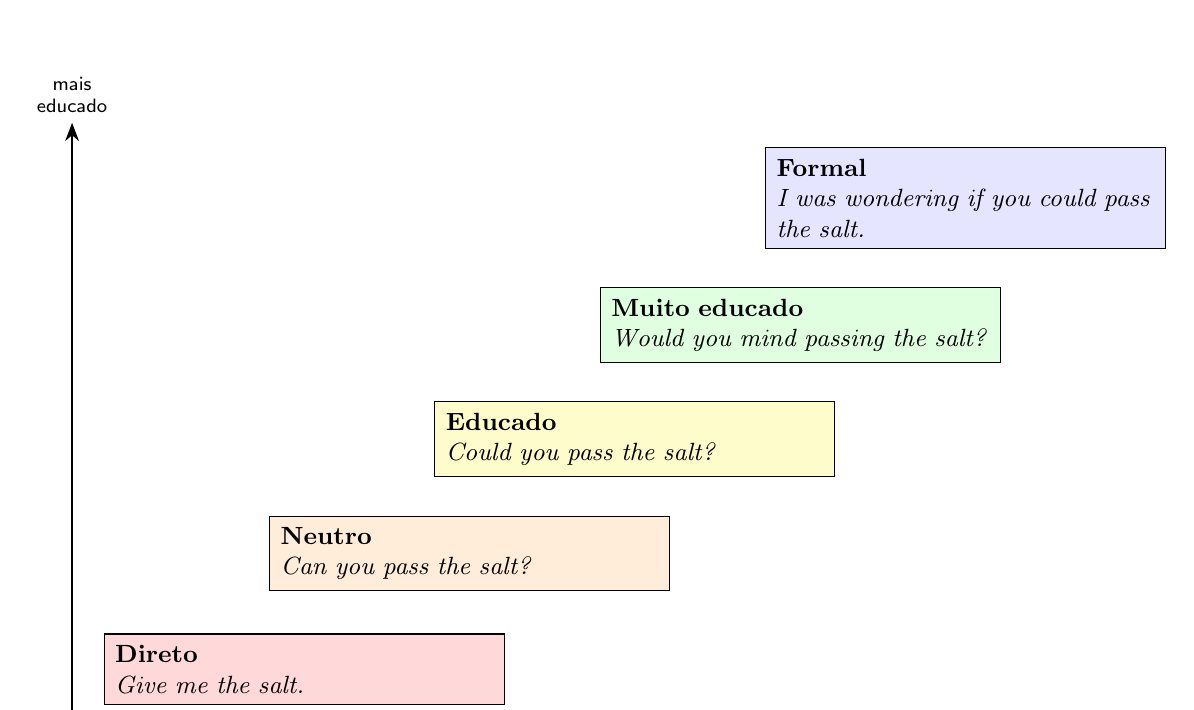
\begin{tikzpicture}
  \foreach \i/\lab/\ex/\col in {
      0/Direto/Give me the salt./red!15,
      1/Neutro/Can you pass the salt?/orange!15,
      2/Educado/Could you pass the salt?/yellow!20,
      3/Muito educado/Would you mind passing the salt?/green!12,
      4/Formal/I was wondering if you could pass the salt./blue!10} {
    \node[draw, fill=\col, anchor=south west, minimum height=0.9cm,
          text width=4.8cm, align=left, font=\small, inner sep=4pt]
      at (\i*2.1, \i*1.45) {\textbf{\lab}\\\textit{\ex}};
  }
  \draw[seta] (-0.4,-0.2) -- (-0.4,7.4) node[above, font=\scriptsize\sffamily, align=center] {mais\\educado};
\end{tikzpicture}
\caption{A escada da polidez: cada degrau acrescenta distância e suavidade.}
\end{figure}

\begin{center}
\begin{tabularx}{\textwidth}{@{}llX@{}}
\toprule
\textbf{Nível} & \textbf{Estrutura} & \textbf{Exemplo} \\
\midrule
Direto & \en{Give me\ldots} & \en{Give me the salt.} (pode soar rude) \\
Neutro & \en{Can you\ldots?} & \en{Can you pass the salt?} \\
Educado & \en{Could you\ldots?} & \en{Could you pass the salt?} \\
Muito educado & \en{Would you mind\ldots?} & \en{Would you mind passing the salt?} \\
Formal & \en{I was wondering if you could\ldots} & \en{I was wondering if you could pass the salt.} \\
\bottomrule
\end{tabularx}
\end{center}

\begin{nota}[Por que \emph{could} é mais educado que \emph{can}?]
\en{Could} e \en{would} são formas ``hipotéticas'' (parecidas com o nosso futuro do pretérito: ``poderia'', ``gostaria''). Soar hipotético dá à outra pessoa espaço para recusar --- e isso é percebido como respeito.
\end{nota}

\section{Pedindo objetos}

\begin{center}
\begin{tabularx}{\textwidth}{@{}lXl@{}}
\toprule
\textbf{Estrutura} & \textbf{Sentido} & \textbf{Exemplo} \\
\midrule
\en{Can I have\ldots?} & Posso ter\ldots? / Me dá\ldots? & \en{Can I have a glass of water?} \\
\en{Could I have\ldots?} & (mais educado) Poderia me dar\ldots? & \en{Could I have the menu, please?} \\
\en{I'd like\ldots}\index{I'd like} & Eu gostaria\ldots & \en{I'd like a coffee, please.} \\
\en{I would like\ldots} & (mais formal) Eu gostaria\ldots & \en{I would like to make a reservation.} \\
\bottomrule
\end{tabularx}
\end{center}

\begin{cuidado}[Atenção: evite ``I want'' para pedir]
Nunca use \en{I want} sozinho para pedir algo a alguém --- soa exigente, quase infantil. Use \en{I'd like} (\en{I'd} = \en{I would}).

\no\ \en{I want a coffee.} \quad \ok\ \en{I'd like a coffee, please.}
\end{cuidado}

\section{Pedindo ações (favores)}

\begin{frases}
\fr{Can you\ldots? \ra\ \en{Can you help me?}}{Você pode\ldots?}
\fr{Could you\ldots? \ra\ \en{Could you open the window?}}{(mais educado) Você poderia\ldots?}
\fr{Would you\ldots? \ra\ \en{Would you please be quiet?}}{Você\ldots? (pedido educado)}
\fr{Would you mind + \textbf{-ing}? \ra\ \en{Would you mind closing the door?}}{Você se importaria de\ldots?}
\end{frases}

\begin{cuidado}[Atenção: \emph{Would you mind\ldots?} se responde com ``No'']
\en{Would you mind}\index{would you mind} significa literalmente ``Você \textbf{se importaria}\ldots?''. Então, para aceitar o pedido, a resposta é \textbf{negativa}:
\begin{itemize}
  \item \en{Would you mind closing the door?} \ra\ \en{\textbf{No}, not at all.} (= não me importo, pode deixar)
  \item Responder \en{Yes} significaria ``sim, eu me importo'' --- ou seja, uma recusa!
\end{itemize}
E o verbo depois de \en{mind} vai sempre no \textbf{gerúndio} (\en{closing}, \en{passing}), nunca \en{to close}.
\end{cuidado}

Sempre que possível, adicione \en{please} no final ou no começo do pedido.

\section{Pedindo permissão}

\begin{center}
\begin{tabularx}{\textwidth}{@{}lXl@{}}
\toprule
\textbf{Estrutura} & \textbf{Registro} & \textbf{Exemplo} \\
\midrule
\en{Can I\ldots?} & Posso\ldots? (informal) & \en{Can I use your phone?} \\
\en{Could I\ldots?} & Poderia\ldots? (educado) & \en{Could I borrow your pen?} \\
\en{May I\ldots?}\index{may} & Posso\ldots? (formal) & \en{May I come in?} \\
\en{Do you mind if I\ldots?} & Você se importa se eu\ldots? & \en{Do you mind if I sit here?} \\
\bottomrule
\end{tabularx}
\end{center}

Note a diferença: \en{Would you mind \textbf{closing}\ldots?} (pede que \emph{a outra pessoa} faça) vs.\ \en{Do you mind \textbf{if I} sit\ldots?} (pede permissão para \emph{você} fazer). As duas seguem a lógica do ``No = pode''.

\section{Pedidos do dia a dia (para memorizar)}

\begin{pratica}[No restaurante]
\begin{frases}
\fr{Could I see the menu, please?}{Posso ver o cardápio, por favor?}
\fr{I'd like the steak, please.}{Eu gostaria do bife, por favor.}
\fr{Can I have the bill, please?}{Pode me trazer a conta, por favor?}
\fr{Could we have some more water?}{Poderia nos trazer mais água?}
\end{frases}
\end{pratica}

\begin{pratica}[Em lojas]
\begin{frases}
\fr{Could you help me, please?}{Você poderia me ajudar, por favor?}
\fr{I'm looking for a jacket.}{Estou procurando uma jaqueta.}
\fr{Can I try this on?}{Posso experimentar?}
\fr{How much is this?}{Quanto custa isto?}
\end{frases}
\end{pratica}

\begin{pratica}[Na rua]
\begin{frases}
\fr{Excuse me, could you tell me where the station is?}{Com licença, poderia me dizer onde fica a estação?}
\fr{Could you take a picture for me?}{Você poderia tirar uma foto para mim?}
\end{frases}
\end{pratica}

\begin{pratica}[No trabalho]
\begin{frases}
\fr{Could you send me that file?}{Você poderia me mandar aquele arquivo?}
\fr{Would you mind reviewing this?}{Você se importaria de revisar isto?}
\fr{Can I ask you a question?}{Posso te fazer uma pergunta?}
\end{frases}
\end{pratica}

\section{Como recusar um pedido (educadamente)}

\begin{frases}
\fr{I'm sorry, I can't.}{Desculpa, não posso.}
\fr{I'm afraid I can't help you.}{Receio que não possa ajudar.}
\fr{I'd love to, but\ldots}{Eu adoraria, mas\ldots}
\fr{Maybe another time.}{Talvez outra hora.}
\fr{Sorry, I'm busy right now.}{Desculpa, estou ocupado(a) agora.}
\end{frases}

\begin{nota}[\emph{I'm afraid\ldots} não é medo]
Em \en{I'm afraid I can't}\index{I'm afraid}, \en{afraid} não tem nada a ver com medo: é um amortecedor educado, equivalente a ``infelizmente'' ou ``receio que''.
\end{nota}

% =====================================================================
\chapter{Como Falar sobre Coisas}
\label{cap:falar}

\section{Descrevendo pessoas, lugares e objetos}

\subsection{A ordem dos adjetivos}

Em inglês, o adjetivo vem \textbf{antes} do substantivo (\en{a red car}, não \en{a car red}). E quando há vários, eles seguem uma ordem fixa\index{ordem dos adjetivos}:

\begin{figure}[H]
\centering
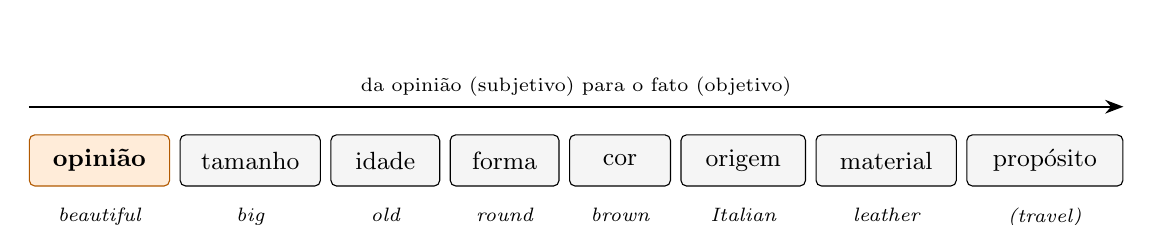
\begin{tikzpicture}[node distance=0.12cm]
  \node[destaque=1.5cm, fill=orange!15, draw=orange!70!black] (o) {opinião};
  \node[caixa=1.5cm, right=of o] (t) {tamanho};
  \node[caixa=1.1cm, right=of t] (i) {idade};
  \node[caixa=1.1cm, right=of i] (f) {forma};
  \node[caixa=1.0cm, right=of f] (c) {cor};
  \node[caixa=1.3cm, right=of c] (g) {origem};
  \node[caixa=1.5cm, right=of g] (m) {material};
  \node[caixa=1.7cm, right=of m] (p) {propósito};
  \foreach \n/\w in {o/beautiful, t/big, i/old, f/round, c/brown, g/Italian, m/leather, p/{(travel)}}
    \node[font=\scriptsize\itshape, below=0.15cm of \n] {\w};
  \draw[seta] ([yshift=0.35cm]o.north west) -- node[above, font=\scriptsize]{da opinião (subjetivo) para o fato (objetivo)} ([yshift=0.35cm]p.north east);
\end{tikzpicture}
\caption{\en{A beautiful big old round brown Italian leather bag.}}
\end{figure}

Na prática, raramente usamos tantos juntos. Mas guarde a ideia central: \textbf{opinião antes de fato}.

\no\ \en{a big nice house} \qquad \ok\ \en{a nice big house}

\subsection{Adjetivos mais usados}

\begin{center}
\begin{tabularx}{\textwidth}{@{}lX@{}}
\toprule
\textbf{Tamanho} & \en{big, small, huge, tiny, medium} \\
\textbf{Idade} & \en{old, new, young, modern, ancient} \\
\textbf{Cor} & \en{red, blue, green, dark, light} \\
\textbf{Aparência} & \en{beautiful, ugly, handsome, pretty, cute} \\
\textbf{Personalidade} & \en{kind, funny, serious, shy, friendly, rude} \\
\textbf{Sensação} & \en{happy, sad, tired, excited, bored, angry} \\
\textbf{Qualidade} & \en{good, bad, great, terrible, amazing, awful} \\
\bottomrule
\end{tabularx}
\end{center}

\begin{nota}[Adjetivo não tem plural]
Diferente do português, o adjetivo em inglês \textbf{nunca} vai para o plural: \en{two big houses} (e não \en{bigs}).
\end{nota}

\subsection{Estruturas}

\estrutura{Sujeito + \emph{to be} + adjetivo}

\begin{frases}
\fr{She is kind.}{Ela é gentil.}
\fr{The food is delicious.}{A comida está deliciosa.}
\end{frases}

\estrutura{Sujeito + verbo + objeto + adjetivo}

\begin{frases}
\fr{I find this book interesting.}{Acho esse livro interessante.}
\end{frases}

\section{Os tempos verbais do dia a dia}

Antes de ver cada tempo, veja onde cada um ``mora'' na linha do tempo\index{tempos verbais}:

\begin{figure}[H]
\centering
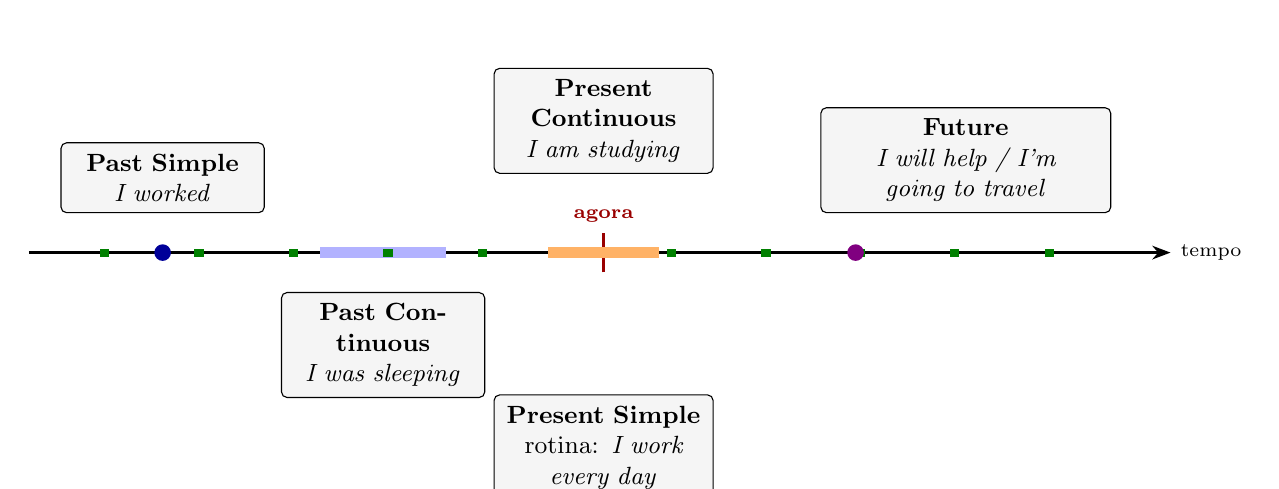
\begin{tikzpicture}
  \draw[seta, thick] (-0.3,0) -- (14.2,0) node[right, font=\scriptsize]{tempo};
  \draw[very thick, red!60!black] (7,-0.25) -- (7,0.25) node[above, font=\scriptsize\bfseries]{agora};
  % past simple
  \fill[blue!60!black] (1.4,0) circle (3pt);
  \node[caixa=2.3cm, above=0.5cm] at (1.4,0) {\textbf{Past Simple}\\\en{I worked}};
  % past continuous
  \draw[line width=4pt, blue!30] (3.4,0) -- (5.0,0);
  \node[caixa=2.3cm, below=0.5cm] at (4.2,0) {\textbf{Past Continuous}\\\en{I was sleeping}};
  % present simple
  \foreach \x in {0.6,1.8,3.0,4.2,5.4,6.6,7.8,9.0,10.2,11.4,12.6} \fill[green!50!black] (\x,-0.05) rectangle ++(0.12,0.1);
  \node[caixa=2.5cm, below=0.5cm] at (7,-1.3) {\textbf{Present Simple}\\rotina: \en{I work every day}};
  % present continuous
  \draw[line width=4pt, orange!60] (6.3,0) -- (7.7,0);
  \node[caixa=2.5cm, above=0.5cm] at (7,0.5) {\textbf{Present Continuous}\\\en{I am studying}};
  % future
  \fill[violet] (10.2,0) circle (3pt);
  \node[caixa=3.4cm, above=0.5cm] at (11.6,0) {\textbf{Future}\\\en{I will help / I'm going to travel}};
\end{tikzpicture}
\caption{Pontos (ações únicas), faixas (ações em progresso) e tracinhos (rotina).}
\end{figure}

\section{Falando do presente}

\subsection{Present Simple --- rotina e fatos}
\index{present simple}

\estrutura{Sujeito + verbo (+ \emph{s/es} na 3ª pessoa do singular)}

\begin{frases}
\fr{I work every day.}{Eu trabalho todo dia.}
\fr{She lives in London.}{Ela mora em Londres.}
\fr{They don't like coffee.}{Eles não gostam de café.}
\fr{He doesn't speak French.}{Ele não fala francês.}
\end{frases}

Na negativa, é a mesma lógica do Capítulo~\ref{cap:perguntas}: \aux{don't/doesn't} + verbo base (\en{He doesn't \textbf{speak}}, não \en{speaks}).

\subsection{Present Continuous --- agora, temporário}
\index{present continuous}

\estrutura{Sujeito + \emph{am/is/are} + verbo-\emph{ing}}

\begin{frases}
\fr{I am studying English.}{Estou estudando inglês.}
\fr{She is working now.}{Ela está trabalhando agora.}
\fr{They aren't sleeping.}{Eles não estão dormindo.}
\end{frases}

\subsection{Marcadores de tempo}

\begin{center}
\begin{tabularx}{\textwidth}{@{}lX@{}}
\toprule
\textbf{Present Simple} & \en{always, usually, often, sometimes, never, every day} \\
\textbf{Present Continuous} & \en{now, right now, at the moment, currently} \\
\bottomrule
\end{tabularx}
\end{center}

\begin{cuidado}[Atenção: o português usa presente para tudo; o inglês não]
``Eu trabalho aqui'' pode ser rotina (\en{I work here}) ou algo temporário (\en{I'm working here this month}). Pergunte-se: \emph{é hábito ou é agora?}
\end{cuidado}

\section{Falando do passado}

\subsection{Past Simple --- ação terminada}
\index{past simple}

\estrutura{Sujeito + verbo no passado (regular \emph{-ed} / irregular)}

\begin{frases}
\fr{I worked yesterday.}{Trabalhei ontem.}
\fr{She went to Paris.}{Ela foi a Paris.}
\fr{They didn't come.}{Eles não vieram.}
\fr{Did you see it?}{Você viu?}
\end{frases}

\subsection{Verbos irregulares mais comuns}
\index{verbos irregulares}

\begin{center}
\begin{tabular}{@{}lll@{\hspace{1.5cm}}lll@{}}
\toprule
\textbf{Base} & \textbf{Passado} & \textbf{Tradução} & \textbf{Base} & \textbf{Passado} & \textbf{Tradução} \\
\midrule
\en{be} & \en{was/were} & ser/estar & \en{think} & \en{thought} & pensar \\
\en{go} & \en{went} & ir & \en{take} & \en{took} & pegar \\
\en{have} & \en{had} & ter & \en{see} & \en{saw} & ver \\
\en{do} & \en{did} & fazer & \en{come} & \en{came} & vir \\
\en{say} & \en{said} & dizer & \en{give} & \en{gave} & dar \\
\en{get} & \en{got} & conseguir & \en{eat} & \en{ate} & comer \\
\en{make} & \en{made} & fazer & \en{drink} & \en{drank} & beber \\
\en{know} & \en{knew} & saber & & & \\
\bottomrule
\end{tabular}
\end{center}

\begin{nota}[Lembrete]
O passado irregular só aparece na \textbf{afirmativa}. Na pergunta e na negativa, o \aux{did} carrega o passado e o verbo volta à base: \en{She \textbf{went}} \ra\ \en{Did she \textbf{go}?} \ra\ \en{She didn't \textbf{go}.}
\end{nota}

\subsection{Past Continuous --- ação em progresso no passado}
\index{past continuous}

\estrutura{Sujeito + \emph{was/were} + verbo-\emph{ing}}

\begin{frases}
\fr{I was sleeping when you called.}{Eu estava dormindo quando você ligou.}
\end{frases}

Ele costuma aparecer junto com o \emph{Past Simple}: a ação longa (\en{was sleeping}) é ``interrompida'' pela curta (\en{called}).

\section{Falando do futuro}
\index{will / going to}

\begin{center}
\begin{tabularx}{\textwidth}{@{}lXX@{}}
\toprule
\textbf{Forma} & \textbf{Quando usar} & \textbf{Estrutura} \\
\midrule
\en{Will} & Decisão espontânea, previsão, promessa & Sujeito + \en{will} + verbo base \\
\en{Going to} & Plano, intenção já decidida & Sujeito + \en{am/is/are going to} + verbo base \\
\en{Present Continuous} & Compromisso marcado (com data/hora) & Sujeito + \en{am/is/are} + verbo-\en{ing} \\
\bottomrule
\end{tabularx}
\end{center}

\begin{frases}
\fr{I will help you.}{Eu vou te ajudar. (decidi agora)}
\fr{It will rain tomorrow.}{Vai chover amanhã. (previsão)}
\fr{I'm going to travel next month.}{Vou viajar mês que vem. (plano)}
\fr{She's going to study medicine.}{Ela vai estudar medicina.}
\fr{I'm meeting her tomorrow.}{Vou encontrá-la amanhã. (marcado)}
\end{frases}

\section{Dando opinião}
\index{opinião}

\begin{pratica}[Frases para opinar]
\begin{frases}
\fr{I think\ldots}{Eu acho\ldots}
\fr{I believe\ldots}{Eu acredito\ldots}
\fr{In my opinion\ldots}{Na minha opinião\ldots}
\fr{From my point of view\ldots}{Do meu ponto de vista\ldots}
\fr{If you ask me\ldots}{Se você me perguntar\ldots}
\fr{To be honest\ldots}{Sendo honesto\ldots}
\fr{Personally, I\ldots}{Pessoalmente, eu\ldots}
\end{frases}
\end{pratica}

Exemplos: \en{I think this movie is amazing.} \,/\, \en{In my opinion, we should wait.} \,/\, \en{To be honest, I don't like it.}

\section{Concordando e discordando}

\begin{center}
\begin{tabularx}{\textwidth}{@{}XXX@{}}
\toprule
\textbf{Concordar} & \textbf{Discordar} & \textbf{Concordar em parte} \\
\midrule
\en{I agree. / I totally agree.} & \en{I don't agree.} & \en{I agree up to a point.} \\
\en{That's true.} & \en{I'm not sure about that.} & \en{You have a point, but\ldots} \\
\en{You're right.} & \en{I see it differently.} & \en{That's true, however\ldots} \\
\en{Exactly!} & \en{That's not how I see it.} & \\
\en{That makes sense.} & \en{I'm afraid I disagree.} & \\
\bottomrule
\end{tabularx}
\end{center}

\section{Falando sobre gostos e preferências}

\begin{frases}
\fr{I like\ldots}{Eu gosto de\ldots}
\fr{I love\ldots}{Eu amo\ldots}
\fr{I enjoy\ldots}{Eu curto\ldots}
\fr{I don't like\ldots}{Eu não gosto de\ldots}
\fr{I hate\ldots}{Eu odeio\ldots}
\fr{I prefer\ldots}{Eu prefiro\ldots}
\fr{I'd rather\ldots}{Eu preferiria\ldots}
\fr{My favorite \blank\ is\ldots}{Meu \blank\ favorito é\ldots}
\end{frases}

Exemplos: \en{I like watching movies.} \,/\, \en{I love Italian food.} \,/\, \en{I'd rather stay home tonight.} \,/\, \en{My favorite color is blue.}

\begin{nota}[Detalhes que fazem diferença]
\begin{itemize}
  \item \en{Like/love/enjoy/hate} + atividade usam \textbf{-ing}: \en{I enjoy \textbf{reading}.} (\en{enjoy} \textbf{só} aceita \emph{-ing}).
  \item \en{I'd rather}\index{I'd rather} + verbo \textbf{base}, sem \en{to}: \en{I'd rather \textbf{stay}}, não \en{to stay}.
  \item \en{Favorite} é a grafia americana; no Reino Unido, \en{favourite}.
\end{itemize}
\end{nota}

% =====================================================================
\chapter{Situações do Dia a Dia}
\label{cap:situacoes}

Este capítulo é um ``kit de sobrevivência'' por situação. Repare como quase tudo aqui é uma aplicação direta dos Capítulos 1--3: perguntas com auxiliar, \en{Could I\ldots?}, \en{I'd like\ldots}.

\section{No restaurante}

\begin{pratica}[Chegando]
\begin{frases}
\fr{A table for two, please.}{Mesa para dois, por favor.}
\fr{Do you have a reservation?}{Vocês têm reserva? (o garçom pergunta)}
\fr{Can we sit outside?}{Podemos sentar do lado de fora?}
\end{frases}
\end{pratica}

\begin{pratica}[Pedindo]
\begin{frases}
\fr{Could I see the menu, please?}{Posso ver o cardápio, por favor?}
\fr{What do you recommend?}{O que você recomenda?}
\fr{I'll have the steak, please.}{Vou querer o bife, por favor.}
\fr{I'd like the chicken, please.}{Eu gostaria do frango, por favor.}
\fr{Can I have it without onions?}{Pode ser sem cebola?}
\fr{Is this spicy?}{Isso é picante?}
\end{frases}
\end{pratica}

\begin{pratica}[Durante a refeição]
\begin{frases}
\fr{Could we have some more water?}{Poderia nos trazer mais água?}
\fr{Excuse me, can I get another fork?}{Com licença, pode me trazer outro garfo?}
\fr{This is delicious!}{Isto está delicioso!}
\end{frases}
\end{pratica}

\begin{pratica}[Pagando]
\begin{frases}
\fr{Can I have the bill, please? (UK) / Check, please. (US)}{A conta, por favor.}
\fr{Do you accept credit cards?}{Aceitam cartão de crédito?}
\fr{Can we split the bill?}{Podemos dividir a conta?}
\fr{Keep the change.}{Fique com o troco.}
\end{frases}
\end{pratica}

\section{No aeroporto}

\begin{frases}
\fr{Where is the check-in counter?}{Onde é o check-in?}
\fr{I'd like a window seat, please.}{Quero um assento na janela, por favor.}
\fr{How many bags are you checking?}{Quantas malas vai despachar?}
\fr{Where is gate B12?}{Onde é o portão B12?}
\fr{Is the flight delayed?}{O voo está atrasado?}
\fr{Where can I find a taxi?}{Onde encontro um táxi?}
\fr{I'm here on vacation / on business.}{Estou aqui de férias / a negócios.}
\fr{I'm staying for a week.}{Vou ficar uma semana.}
\end{frases}

\begin{nota}[Na imigração]
As duas últimas frases respondem às perguntas clássicas do agente de imigração: \en{What's the purpose of your visit?} (motivo da visita) e \en{How long are you staying?} (quanto tempo vai ficar).
\end{nota}

\section{No hotel}

\begin{frases}
\fr{I have a reservation under [name].}{Tenho reserva no nome de\ldots}
\fr{I'd like to check in, please.}{Gostaria de fazer o check-in, por favor.}
\fr{What time is check-out?}{Que horas é o check-out?}
\fr{Is breakfast included?}{O café da manhã está incluso?}
\fr{Could I have a wake-up call at 7?}{Pode me acordar às 7?}
\fr{The air conditioner isn't working.}{O ar-condicionado não está funcionando.}
\fr{Could I have extra towels?}{Pode mandar toalhas extras?}
\fr{Can I leave my luggage here?}{Posso deixar minha mala aqui?}
\end{frases}

\section{Fazendo compras}

\begin{frases}
\fr{How much is this?}{Quanto custa isso?}
\fr{Do you have this in another size/color?}{Tem em outro tamanho/cor?}
\fr{Can I try this on?}{Posso experimentar?}
\fr{Where is the fitting room?}{Onde é o provador?}
\fr{I'm just looking, thanks.}{Só estou olhando, obrigado(a).}
\fr{Do you have a smaller/larger size?}{Tem tamanho menor/maior?}
\fr{Is there a discount?}{Tem desconto?}
\fr{I'll take it.}{Vou levar.}
\fr{Can I pay by card?}{Posso pagar com cartão?}
\fr{Could I have a receipt?}{Pode me dar o recibo?}
\end{frases}

\section{No médico / na farmácia}

\begin{frases}
\fr{I don't feel well.}{Não estou me sentindo bem.}
\fr{I have a headache.}{Estou com dor de cabeça.}
\fr{I have a sore throat.}{Estou com dor de garganta.}
\fr{I have a fever.}{Estou com febre.}
\fr{I have a stomachache.}{Estou com dor de barriga.}
\fr{I'm allergic to penicillin.}{Sou alérgico(a) a penicilina.}
\fr{I need a doctor.}{Preciso de um médico.}
\fr{Where is the nearest pharmacy?}{Onde é a farmácia mais próxima?}
\fr{Do I need a prescription?}{Preciso de receita?}
\fr{How often should I take this?}{Com que frequência devo tomar isso?}
\end{frases}

\begin{nota}[Padrão: ``estar com'' dor $\to$ \emph{have}]
Onde o português diz ``estou \textbf{com} dor/febre'', o inglês usa \en{I \textbf{have} a\ldots}. Nunca \en{I'm with a headache}. O mesmo vale para o erro \en{I'm with hunger} (Capítulo~\ref{cap:erros}).
\end{nota}

\section{No trabalho}

\begin{frases}
\fr{Can I ask you a question?}{Posso te fazer uma pergunta?}
\fr{Could you send me that file?}{Pode me enviar aquele arquivo?}
\fr{I'll get back to you.}{Eu te retorno.}
\fr{Let me know if you need anything.}{Me avise se precisar de algo.}
\fr{I'm working on it.}{Estou trabalhando nisso.}
\fr{Can we schedule a meeting?}{Podemos agendar uma reunião?}
\fr{I'm sorry, I'm running late.}{Desculpa, estou atrasado(a).}
\fr{Could you clarify that?}{Pode esclarecer isso?}
\end{frases}

\section{Small talk (conversa fiada)}
\index{small talk}

\begin{frases}
\fr{How's the weather today?}{Como está o tempo hoje?}
\fr{Did you watch the game last night?}{Você assistiu ao jogo ontem?}
\fr{How was your weekend?}{Como foi seu fim de semana?}
\fr{What are you doing this weekend?}{O que você vai fazer neste fim de semana?}
\fr{Have you seen this movie?}{Você viu esse filme?}
\fr{I love this city.}{Adoro essa cidade.}
\end{frases}

Note \en{What \textbf{are} you \textbf{doing} this weekend?}: é o \emph{Present Continuous} com valor de futuro, pedindo os planos já combinados.

% =====================================================================
\chapter{Erros Comuns de Brasileiros}
\label{cap:erros}

A maioria desses erros vem de \textbf{traduzir palavra por palavra} do português. Por isso eles são tão comuns --- e tão fáceis de corrigir depois que você os enxerga.

\section{Erros de estrutura}

\begin{center}
\begin{tabularx}{\textwidth}{@{}p{3.6cm}p{3.6cm}X@{}}
\toprule
\textbf{\no\ Errado} & \textbf{\ok\ Certo} & \textbf{Explicação} \\
\midrule
\en{I have 25 years.} & \en{I am 25 years old.} & Idade usa \en{to be} \\
\en{I'm agree.} & \en{I agree.} & \en{Agree} já é verbo \\
\en{I go to home.} & \en{I go home.} & \en{Home} não leva \en{to} (depois de verbos de movimento) \\
\en{People is\ldots} & \en{People are\ldots} & \en{People} é plural \\
\en{Explain me.} & \en{Explain to me.} & \en{Explain} pede \en{to} \\
\en{I'm boring.} & \en{I'm bored.} & \en{boring} = chato; \en{bored} = entediado \\
\en{Make a question.} & \en{Ask a question.} & Pergunta se ``faz'' com \en{ask} \\
\en{I did a mistake.} & \en{I made a mistake.} & Erro se ``faz'' com \en{make} \\
\en{I have a doubt.} & \en{I have a question.} & \en{Doubt} = dúvida no sentido de desconfiança \\
\en{I'm with hunger.} & \en{I'm hungry.} & Fome é adjetivo \\
\en{I'm with cold.} & \en{I'm cold.} & Frio é adjetivo \\
\en{How is called?} & \en{What is it called?} & Precisa de sujeito (\en{it}) e usa \en{what} \\
\en{Since 2 years.} & \en{For 2 years.} & \en{For} = duração; \en{since} = ponto de início (\en{since 2020}) \\
\bottomrule
\end{tabularx}
\end{center}

\begin{cuidado}[Atenção: \emph{-ing} descreve, \emph{-ed} sente]
\en{I'm boring} significa ``eu sou uma pessoa chata''. Regra geral\index{boring / bored}: adjetivo em \textbf{-ing} descreve \emph{o que causa} o sentimento; em \textbf{-ed}, \emph{quem sente}.
\begin{itemize}
  \item \en{The movie is boring.} \ra\ \en{I'm bored.}
  \item \en{The news is exciting.} \ra\ \en{I'm excited.}
  \item \en{This is confusing.} \ra\ \en{I'm confused.}
\end{itemize}
\end{cuidado}

\begin{nota}[\emph{Explain} + \emph{to}]
A ordem mais natural é colocar a coisa explicada primeiro: \en{Can you explain \textbf{this} to me?} Nunca \en{explain me}.
\end{nota}

\section{Falsos amigos (\emph{false friends})}
\index{falsos amigos}

Palavras que parecem com o português, mas significam outra coisa:

\begin{center}
\begin{tabularx}{\textwidth}{@{}lXX@{}}
\toprule
\textbf{Palavra} & \textbf{Significa de verdade} & \textbf{Para dizer o ``português''} \\
\midrule
\en{actually}\index{actually} & na verdade & atualmente = \en{currently} \\
\en{pretend} & fingir & pretender = \en{intend} \\
\en{push} & empurrar & puxar = \en{pull} (cuidado nas portas!) \\
\en{library} & biblioteca & livraria = \en{bookstore} \\
\en{parents} & pais (pai e mãe) & parentes = \en{relatives} \\
\bottomrule
\end{tabularx}
\end{center}

% =====================================================================
\chapter{Vocabulário e Frases Essenciais}
\label{cap:vocabulario}

\section{Cumprimentos e despedidas}

\begin{frases}
\fr{Hello / Hi / Hey}{Olá / Oi / Ei}
\fr{Good morning / afternoon / evening}{Bom dia / boa tarde / boa noite (ao chegar)}
\fr{Good night}{Boa noite (ao dormir ou ir embora)}
\fr{How are you?}{Como você está?}
\fr{Nice to meet you.}{Prazer em conhecer.}
\fr{See you later.}{Até mais.}
\fr{Take care.}{Se cuida.}
\fr{Have a nice day.}{Tenha um bom dia.}
\fr{Goodbye / Bye.}{Tchau.}
\end{frases}

\begin{cuidado}[Atenção: \emph{good evening} $\neq$ \emph{good night}]
\en{Good evening} é cumprimento de \textbf{chegada} à noite. \en{Good night} é \textbf{despedida}. Chegar num restaurante dizendo \en{Good night!} soa como se você já estivesse indo embora.
\end{cuidado}

\section{Números, datas e horas}

\begin{center}
\begin{tabularx}{\textwidth}{@{}lX@{}}
\toprule
\textbf{Números} & \en{one, two, three\ldots\ ten, twenty, thirty, hundred, thousand, million} \\
\textbf{Dias} & \en{Monday, Tuesday, Wednesday, Thursday, Friday, Saturday, Sunday} \\
\textbf{Meses} & \en{January, February, March, April, May, June, July, August, September, October, November, December} \\
\bottomrule
\end{tabularx}
\end{center}

Dias e meses são escritos \textbf{com letra maiúscula} em inglês.

\textbf{Horas:} \en{What time is it?} \ra\ \en{It's 3 o'clock.} (3h) / \en{It's half past two.} (2h30) / \en{It's a quarter to five.} (4h45)

\begin{figure}[H]
\centering
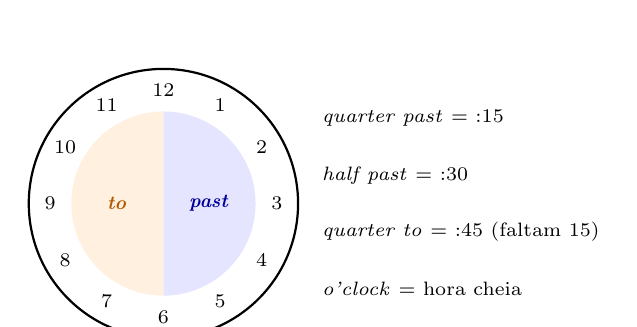
\begin{tikzpicture}[scale=0.9]
  \draw[thick] (0,0) circle (1.9);
  \foreach \h in {1,...,12} \node[font=\scriptsize] at ({90-30*\h}:1.6) {\h};
  \fill[blue!10] (0,0) -- (90:1.3) arc (90:-90:1.3) -- cycle;
  \fill[orange!12] (0,0) -- (-90:1.3) arc (270:90:1.3) -- cycle;
  \node[font=\scriptsize\bfseries, text width=1.4cm, align=center, blue!60!black] at (0.65,0) {\en{past}};
  \node[font=\scriptsize\bfseries, text width=1.4cm, align=center, orange!70!black] at (-0.65,0) {\en{to}};
  \node[font=\scriptsize, right] at (2.1,1.2) {\en{quarter past} = :15};
  \node[font=\scriptsize, right] at (2.1,0.4) {\en{half past} = :30};
  \node[font=\scriptsize, right] at (2.1,-0.4) {\en{quarter to} = :45 (faltam 15)};
  \node[font=\scriptsize, right] at (2.1,-1.2) {\en{o'clock} = hora cheia};
\end{tikzpicture}
\caption{Metade direita do relógio: \en{past} (``e\ldots''); metade esquerda: \en{to} (``para as\ldots'').}
\end{figure}

\section{Palavras de ligação (conectivos)}
\index{conectivos}

\begin{center}
\begin{tabular}{@{}ll@{\hspace{2cm}}ll@{}}
\toprule
\en{and} & e & \en{also} & também \\
\en{but} & mas & \en{however} & no entanto \\
\en{or} & ou & \en{although} & embora \\
\en{so} & então & \en{therefore} & portanto \\
\en{because} & porque & & \\
\bottomrule
\end{tabular}
\end{center}

\section{Frases de emergência}

\begin{pratica}[Guarde estas de cor]
\begin{frases}
\fr{Help!}{Socorro!}
\fr{Call the police!}{Chame a polícia!}
\fr{I need an ambulance.}{Preciso de uma ambulância.}
\fr{I'm lost.}{Estou perdido(a).}
\fr{I lost my passport.}{Perdi meu passaporte.}
\fr{Where is the embassy?}{Onde é a embaixada?}
\fr{I don't speak English very well.}{Não falo inglês muito bem.}
\fr{Do you speak Portuguese?}{Você fala português?}
\fr{Can you help me?}{Pode me ajudar?}
\end{frases}
\end{pratica}

\section{Frases para ``ganhar tempo'' na conversa}

\begin{frases}
\fr{Well\ldots}{Bem\ldots}
\fr{Let me think.}{Deixa eu pensar.}
\fr{That's a good question.}{Boa pergunta.}
\fr{How can I say this\ldots}{Como posso dizer isso\ldots}
\fr{What I mean is\ldots}{O que quero dizer é\ldots}
\fr{In other words\ldots}{Em outras palavras\ldots}
\end{frases}

\section{Saudações formais (e-mail / carta)}

\begin{frases}
\fr{Dear Mr. Smith,}{Prezado Sr. Smith,}
\fr{I hope this email finds you well.}{Espero que esteja bem.}
\fr{I'm writing to\ldots}{Escrevo para\ldots}
\fr{Best regards,}{Atenciosamente,}
\fr{Sincerely,}{Cordialmente, (fecho formal)}
\end{frases}

\begin{nota}[\emph{Sincerely} não é ``sinceramente'' aqui]
Como fecho de carta, \en{Sincerely} (ou \en{Yours sincerely}, no Reino Unido) equivale ao nosso ``Cordialmente'' / ``Atenciosamente'' --- é só uma fórmula de encerramento formal.
\end{nota}

% =====================================================================
\chapter{Exercícios Práticos com Gabarito}
\label{cap:exercicios}

Faça cada bloco \textbf{sem olhar} o gabarito, que está no fim do capítulo. Se errar, volte à seção indicada entre parênteses.

\section{Transforme em perguntas \emph{Yes/No} (Seção 1.2)}
\begin{enumerate}
  \item \en{You like pizza.} \ra\ \blank\blank\blank
  \item \en{She works here.} \ra\ \blank\blank\blank
  \item \en{They went home.} \ra\ \blank\blank\blank
  \item \en{He can swim.} \ra\ \blank\blank\blank
  \item \en{You are tired.} \ra\ \blank\blank\blank
\end{enumerate}

\section{Complete com o auxiliar correto (Seção 1.2)}
\begin{enumerate}
  \item \blank\ \en{you speak English?}
  \item \blank\ \en{she like coffee?}
  \item \blank\ \en{they go to the party?} (ontem)
  \item \blank\ \en{he a teacher?}
  \item \blank\ \en{you seen this movie?}
\end{enumerate}

\section{Traduza para o inglês (Capítulos 1 e 3)}
\begin{enumerate}
  \item Onde você mora?
  \item Você pode me ajudar?
  \item Eu gostaria de um café, por favor.
  \item Quantos anos você tem?
  \item Você poderia repetir, por favor?
\end{enumerate}

\section{Responda com \emph{short answers} (Seção 2.1)}
\begin{enumerate}
  \item \en{Do you like chocolate?} (sim) \ra\ \blank\blank
  \item \en{Did you sleep well?} (não) \ra\ \blank\blank
  \item \en{Can you drive?} (sim) \ra\ \blank\blank
  \item \en{Are you married?} (não) \ra\ \blank\blank
  \item \en{Have you been to London?} (não) \ra\ \blank\blank
\end{enumerate}

\section{Corrija os erros (Capítulo 6)}
\begin{enumerate}
  \item \en{I have 30 years.}
  \item \en{I'm agree with you.}
  \item \en{Explain me this.}
  \item \en{People is nice here.}
  \item \en{I'm boring.} (querendo dizer ``estou entediado'')
\end{enumerate}

\section{Complete com o tempo verbal correto (Capítulo 4)}
\begin{enumerate}
  \item \en{I} \blank\ \en{(study) English every day.}
  \item \en{She} \blank\ \en{(work) right now.}
  \item \en{They} \blank\ \en{(go) to Paris last year.}
  \item \en{We} \blank\ \en{(travel) next month.}
  \item \en{He} \blank\ \en{(not / like) coffee.}
\end{enumerate}

\newpage
\section{Gabarito}

\begin{center}
\small
\begin{tabularx}{\textwidth}{@{}lXXX@{}}
\toprule
& \textbf{8.1 Perguntas} & \textbf{8.2 Auxiliares} & \textbf{8.3 Tradução} \\
\midrule
1 & \en{Do you like pizza?} & \en{Do} & \en{Where do you live?} \\
2 & \en{Does she work here?} & \en{Does} & \en{Can you help me?} \\
3 & \en{Did they go home?} & \en{Did} & \en{I'd like a coffee, please.} \\
4 & \en{Can he swim?} & \en{Is} & \en{How old are you?} \\
5 & \en{Are you tired?} & \en{Have} & \en{Could you repeat that, please?} \\
\bottomrule
\end{tabularx}

\vspace{1em}
\begin{tabularx}{\textwidth}{@{}lXXX@{}}
\toprule
& \textbf{8.4 Short answers} & \textbf{8.5 Correções} & \textbf{8.6 Tempos verbais} \\
\midrule
1 & \en{Yes, I do.} & \en{I am 30 years old.} & \en{study} \\
2 & \en{No, I didn't.} & \en{I agree with you.} & \en{is working} \\
3 & \en{Yes, I can.} & \en{Explain this to me.} & \en{went} \\
4 & \en{No, I'm not.} & \en{People are nice here.} & \en{are going to travel / will travel} \\
5 & \en{No, I haven't.} & \en{I'm bored.} & \en{doesn't like} \\
\bottomrule
\end{tabularx}
\end{center}

\begin{nota}[Comentários sobre o gabarito]
\begin{itemize}
  \item \textbf{8.2, item 3:} sem contexto, \en{Do they go to the party?} (rotina) também seria gramatical; com ``ontem'', só \en{Did}.
  \item \textbf{8.2, item 5:} \en{seen} é particípio, então o auxiliar precisa ser \en{have} (\emph{present perfect}).
  \item \textbf{8.6, item 4:} \en{are going to travel} é o mais natural para um plano; \en{We're traveling next month} (compromisso marcado) também está certo.
\end{itemize}
\end{nota}

% =====================================================================
\chapter{Resumo Final --- As 10 Regras de Ouro}
\label{cap:revisao}

\begin{enumerate}
  \item Toda pergunta em inglês precisa de \textbf{estrutura}, não só entonação.
  \item Sim/Não \ra\ use \textbf{auxiliar} (\en{do/does/did/am/is/are/will/can}\ldots).
  \item \emph{WH- questions}: \textbf{WH + auxiliar + sujeito + verbo}.
  \item Respostas curtas são a norma: \en{Yes, I do.} / \en{No, I don't.}
  \item Nunca responda só ``\en{Yes}'' ou ``\en{No}'' --- pode soar rude.
  \item Pedidos educados: \en{Could you\ldots?} / \en{I'd like\ldots} / \en{Would you mind\ldots?}
  \item Nunca use \en{I want} para pedir --- use \en{I'd like}.
  \item \en{Actually} = na verdade, não ``atualmente''.
  \item Cuidado com falsos amigos (\en{pretend} $\neq$ pretender, \en{push} $\neq$ puxar).
  \item Errou? Não entendeu? Peça: \en{Sorry, could you repeat that?}
\end{enumerate}

\section{Qual auxiliar usar? (fluxograma)}

Este é o raciocínio que você aplica, em segundos, antes de qualquer pergunta, negativa, resposta curta ou \emph{question tag}:

\begin{figure}[H]
\centering
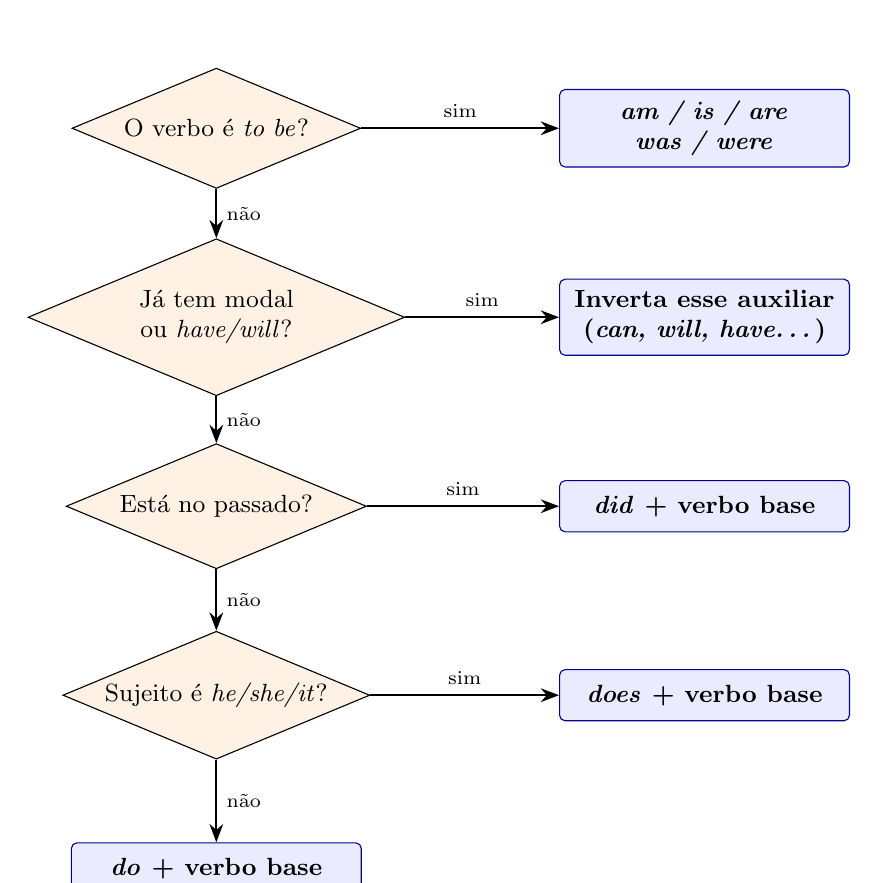
\begin{tikzpicture}[
    decisao/.style={draw, diamond, aspect=2.4, fill=orange!10, align=center, font=\small, inner sep=1pt, text width=2.9cm},
    fim/.style={destaque=3.4cm},
  ]
  \node[decisao] (d1) at (0,0) {O verbo é \en{to be}?};
  \node[fim] (r1) at (6.2,0) {\en{am / is / are}\\\en{was / were}};
  \node[decisao] (d2) at (0,-2.4) {Já tem modal ou \en{have/will}?};
  \node[fim] (r2) at (6.2,-2.4) {Inverta esse auxiliar\\(\en{can, will, have\ldots})};
  \node[decisao] (d3) at (0,-4.8) {Está no passado?};
  \node[fim] (r3) at (6.2,-4.8) {\en{did} + verbo base};
  \node[decisao] (d4) at (0,-7.2) {Sujeito é \en{he/she/it}?};
  \node[fim] (r4) at (6.2,-7.2) {\en{does} + verbo base};
  \node[fim] (r5) at (0,-9.4) {\en{do} + verbo base};

  \draw[seta] (d1) -- node[above, font=\scriptsize]{sim} (r1);
  \draw[seta] (d2) -- node[above, font=\scriptsize]{sim} (r2);
  \draw[seta] (d3) -- node[above, font=\scriptsize]{sim} (r3);
  \draw[seta] (d4) -- node[above, font=\scriptsize]{sim} (r4);
  \draw[seta] (d1) -- node[right, font=\scriptsize]{não} (d2);
  \draw[seta] (d2) -- node[right, font=\scriptsize]{não} (d3);
  \draw[seta] (d3) -- node[right, font=\scriptsize]{não} (d4);
  \draw[seta] (d4) -- node[right, font=\scriptsize]{não} (r5);
\end{tikzpicture}
\caption{Escolhendo o auxiliar certo.}
\end{figure}

\section{As cinco estruturas do guia}

\begin{center}
\begin{tabularx}{\textwidth}{@{}lXl@{}}
\toprule
\textbf{Estrutura} & \textbf{Fórmula} & \textbf{Exemplo} \\
\midrule
Yes/No question & Aux + Sujeito + Verbo? & \en{Does he work here?} \\
WH- question & WH + Aux + Sujeito + Verbo? & \en{Where do you live?} \\
Short answer & Yes/No + Sujeito + Aux & \en{Yes, he does.} \\
Question tag & Frase (+/$-$), Aux oposto + Pronome? & \en{You're tired, aren't you?} \\
Indirect question & Introdução + WH + Sujeito + Verbo & \en{Do you know where he lives?} \\
\bottomrule
\end{tabularx}
\end{center}

% =====================================================================
\appendix
\chapter{Referências e Leitura Adicional}

\begin{itemize}
  \item \textbf{Raymond Murphy}, \emph{English Grammar in Use} (Cambridge University Press) --- unidades sobre \emph{questions}, \emph{auxiliary verbs}, \emph{question tags} e \emph{short answers}. A referência clássica para autoestudo (a versão \emph{Essential Grammar in Use} é para iniciantes).
  \item \textbf{Michael Swan}, \emph{Practical English Usage} (Oxford University Press) --- verbetes sobre \emph{questions}, \emph{indirect speech}, \emph{requests} e polidez.
  \item \textbf{Cambridge Dictionary --- Grammar}: \url{https://dictionary.cambridge.org/grammar/british-grammar/} (seções \emph{Questions}, \emph{Question tags}, \emph{Politeness}).
  \item \textbf{British Council --- LearnEnglish}: \url{https://learnenglish.britishcouncil.org/} --- explicações gratuitas e exercícios interativos de gramática por nível.
  \item \textbf{Cambridge Dictionary} (com áudio de pronúncia britânica e americana): \url{https://dictionary.cambridge.org/}.
\end{itemize}

\chapter{Glossário}

\begin{description}
  \item[Auxiliar\index{auxiliar}] Verbo ``ajudante'' (\en{do, does, did, be, have, will, can}\ldots) que carrega tempo e pessoa e se move para antes do sujeito nas perguntas.
  \item[Forma base\index{forma base}] O verbo sem nenhuma terminação (\en{work, call, go}). Usada depois de \en{do/does/did} e de modais.
  \item[Falso amigo\index{falsos amigos}] Palavra parecida com o português mas com outro significado (\en{actually}, \en{pretend}, \en{library}, \en{parents}).
  \item[Going to\index{will / going to}] Futuro de plano ou intenção já decidida (\en{I'm going to travel}).
  \item[Indirect question\index{indirect question}] Pergunta embutida numa frase introdutória (\en{Could you tell me\ldots}); mantém a ordem de afirmação.
  \item[Inversão\index{inversão}] Troca de posição entre sujeito e auxiliar: \en{She is} \ra\ \en{Is she?}
  \item[Modal verb\index{modal verb}] Auxiliares como \en{can, could, will, would, should, may, might, must}; nunca recebem \en{-s} e são seguidos da forma base.
  \item[Past Continuous\index{past continuous}] \en{was/were} + verbo-\en{ing}; ação em progresso no passado.
  \item[Past Simple\index{past simple}] Passado de ação terminada (\en{-ed} ou forma irregular).
  \item[Present Continuous\index{present continuous}] \en{am/is/are} + verbo-\en{ing}; ação acontecendo agora ou temporária.
  \item[Pergunta de sujeito\index{pergunta de sujeito}] Pergunta em que \en{who}/\en{what} é o próprio sujeito (\en{Who called you?}); não usa \en{do/does/did}.
  \item[Present perfect\index{present perfect}] \en{have/has} + particípio (\en{Have you seen it?}); liga passado e presente.
  \item[Present Simple\index{present simple}] Presente de rotina e fatos; ganha \en{-s} na 3ª pessoa do singular.
  \item[Question tag\index{question tag}] Mini-pergunta no fim da frase para pedir confirmação, com polaridade oposta (\en{\ldots, aren't you?}).
  \item[Request\index{request}] Pedido de objeto, ação ou permissão, normalmente com forma de pergunta.
  \item[Short answer\index{short answer}] Resposta curta com \en{Yes/No} + sujeito + auxiliar (\en{Yes, I do}).
  \item[Small talk\index{small talk}] Conversa leve e social (tempo, fim de semana, ``como vai'') que abre interações.
  \item[WH- question\index{WH- question}] Pergunta iniciada por \en{what, where, when, who, why, which, how}\ldots, que pede uma informação.
  \item[Yes/No question\index{Yes/No question}] Pergunta cuja resposta é sim ou não, formada com auxiliar antes do sujeito.
\end{description}

\printindex

\end{document}
